\documentclass{article}

\usepackage{graphicx}
\usepackage{verbatim}
\usepackage{placeins}
\usepackage{hyperref}
\usepackage{tikz}
\usepackage{minted}
\usepackage{amsmath}

\usetikzlibrary{positioning}

\graphicspath{ {./images/} }

\begin{document}

\title{Cicada 3301 - 2012 "everywhere" images analysis}
\author{tweqx} % Credit yourself here! author1 \and author2 \and author3 \and ...
\date{December 2022}
\maketitle

\begin{abstract}
	{\color{red} TODO}
\end{abstract}

\section{Introduction}

Back in 2012, during the first edition of the Cicada 3301 puzzle, solvers were given a list of coordinates after numerous puzzle steps. A QR code could be found in most locations, linking to an URL of the form:
\begin{center}
	\texttt{http://845145127.com/}\textit{numbers}\texttt{.jpg}
\end{center}

\noindent where each QR code found had a different sequence "\textit{numbers}".

Two different JPG images could be found at these URLs: they both consisted of an overexposed Cicada 3301 logo on a black background. The group name could be found beneath this logo, along with the omnious message "everywhere" placed above.

\begin{figure}[h]
	\centering
	
	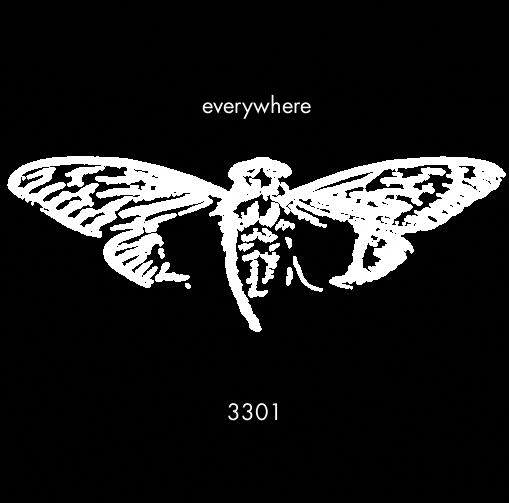
\includegraphics[scale=0.3]{agrippa}
	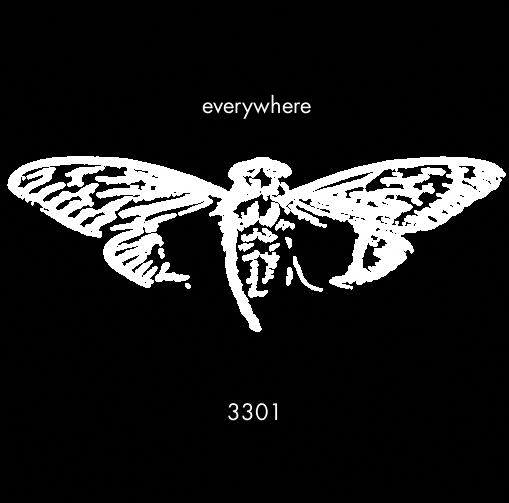
\includegraphics[scale=0.3]{brittanica}
	
	\caption{The two "everywhere" images}
\end{figure}

While they looked exactly the same, a different PGP-signed message was steganographically hidden within each variant.

\begin{figure}[h]
	\centering
	\tiny

	\begin{minipage}{0.5\textwidth}
		\verbatiminput{data/agrippa.asc}	
	\end{minipage}%
	\begin{minipage}{0.5\textwidth}
		\verbatiminput{data/brittanica.asc}
	\end{minipage}

	\caption{The two PGP-signed messages found}
\end{figure}
\FloatBarrier

The poems found in these messages hinted the book needed to complete the associated book code. For respectively each of the message above, they were "\textit{Agrippa (A Book of the Dead)}" by William Gibson and the "\textit{Encyclop\ae{}dia Brittanica}".

When deciphered, each book code led to an Tor address, allowing for further progress. \\

Unfortunately, the two "Everywhere" variants weren't properly archived.

The furthest archive of the "Agrippa" variant can be found on the wiki, added by Lurker69 in 2014 : \href{https://static.wikia.nocookie.net/uncovering-cicada/images/c/cd/Everyehere.jpg}{everywhere}.

For many years, no copy of the "Brittanica" variant was known. One copy recently surfaced when optimisticninja's gitlab repository was made public%
%
\footnote{\url{https://gitlab.com/optimisticninja/cicada3301/}, \texttt{2012/03.subreddit/04.qr\_codes}\\
	Archive :  \url{https://github.com/cicada-solvers/optimisticninja_cicada3301}}%
%
. No source that could justify where it originates from is provided. Furthermore, this same repository is known to contain fake assets, such as a fake screenshot of the countdown found on \texttt{845145127.com}. \\

This analysis aims at investigating the two archives of the "everywhere" to try to determine whether or not they are legitimate.

\section{Goals and methodology}

The upstream Outguess version in 2012 was Outguess v0.2. For this reason, we'll use its source code as the base of our analysis. \href{https://fossies.org/linux/privat/old/outguess-0.2.tar.gz/}{Source code}. \\

Readers should be familiar with the encoding of JPEG: what are Discrete Cosine Transforms coefficients, how are they used...

\section{Inner workings of Outguess}

\subsection{General principles}

To steganographically hide a message in an image, Outguess follows a serie of general steps. They have been highlighted in Outguess' \texttt{main} function, simplified below:

\begin{minted}[fontsize=\footnotesize]{C}
int
main(int argc, char **argv)
{
	// ...
	
	/* read command line arguments */
	while ((ch = getopt(argc, argv, "eErmftp:s:S:i:I:k:d:D:K:x:F:")) != -1)
		// ...
	}
	
	// `doretrieve` corresponds to the flag -r
	
	
	argc -= optind;
	argv += optind;
	
	// ...
	
	if (argc == 2) {
		srch = get_handler(argv[0]);
		if (srch == NULL) {
			fprintf(stderr, "Unknown data type of %s\n", argv[0]);
			exit (1);
		}
		if (!doretrieve) {
			// expect the second argument to be the output image name
			
			dsth = get_handler(argv[1]);
			if (dsth == NULL) {
				fprintf(stderr, "Unknown data type of %s\n",
				argv[1]);
				exit (1);
			}
		}
		fin = fopen(argv[0], "rb");
		// ...
		fout = fopen(argv[1], "wb");
		// ...
	} else {
		// read/write from stdin/stdout
		// ...
	}
	
	/* Initialize Golay-Tables for 12->23 bit error correction */
	// ...
	
	fprintf(stderr, "Reading %s....\n", argv[0]);
	image = srch->read(fin);
	
	if (extractonly) {
		// Special mode, only available iif the outguess executable is named "extract"
		// Usage : extract image.jpg output_file.txt
		
		int bits;
		/* Wen extracting get the bitmap from the source handler */
		srch->get_bitmap(&bitmap, image, STEG_RETRIEVE);
		
		fprintf(stderr, "Writing %d bits\n", bitmap.bits);
		bits = htonl(bitmap.bits);
		fwrite(&bits, 1, sizeof(int), fout);
		fwrite(bitmap.bitmap, bitmap.bytes, sizeof(char), fout);
		exit (1);
	} else if (doretrieve)
		// -r

		/* Wen extracting get the bitmap from the source handler */
		srch->get_bitmap(&bitmap, image, STEG_RETRIEVE);
	else {
		/* Initialize destination data handler */
		dsth->init(param);
		/* When embedding the destination format determines the bits */
		dsth->get_bitmap(&bitmap, image, 0);
	}
	fprintf(stderr, "Extracting usable bits:   %d bits\n", bitmap.bits);
	
	// -e
	if (doerror)
		cfg1.flags |= STEG_ERROR;
	
	if (!doretrieve) {
		// hide message in image

		// -m
		if (mark)
			cfg1.flags |= STEG_MARK;

		// -F ('on' by default)
		if (foil) {
			dsth->preserve(&bitmap, -1);
			
			if (bitmap.maxcorrect)
				fprintf(stderr,
					"Correctable message size: %d bits, %0.2f%%\n",
					bitmap.maxcorrect,
					(float)100*bitmap.maxcorrect/bitmap.bits);
		}
		
		do_embed(&bitmap, data, key, strlen(key), &cfg1, &cumres);
		
		// outguess can embed up to two messages (a key has to be used for the second message though)
		if (key2 && data2) {
			// ... embed the second file
		}
		
		if (foil) {
			// ...
			
			memset(steg_offset, 0, sizeof(steg_offset));
			steg_foil = steg_foilfail = 0;
			
			for (i = 0; i < bitmap.bits; i++) {
				if (!TEST_BIT(plocked, i))
				continue;
				
				cbit = TEST_BIT(pbits, i) ? 1 : 0;
				
				if (cbit == (data[i] & 0x01))
				continue;
				
				n = bitmap.preserve(&bitmap, i);
				if (n > 0) {
					/* Actual modificaton */
					n = abs(n - i);
					if (n > MAX_SEEK)
					n = MAX_SEEK;
					
					steg_offset[n - 1]++;
				}
			}
			
			/* Indicates that we are done with the image */
			bitmap.preserve(&bitmap, bitmap.bits);
			
			/* Calculate statistics */
			// ... mean
			// ... stddev
			
			fprintf(stderr, "Foiling statistics: "
				"corrections: %d, failed: %d, "
				"offset: %f +- %f\n",
				steg_foil, steg_foilfail,
				mean, sqrt(dev / (count - 1)));
		}
		
		fprintf(stderr, "Total bits changed: %d (change %d + bias %d)\n",
			cumres.changed + cumres.bias,
			cumres.changed, cumres.bias);
		fprintf(stderr, "Storing bitmap into data...\n");
		
		dsth->put_bitmap (image, &bitmap, cfg1.flags);
		
		#ifdef FOURIER
		// -f
		if (dofourier)
			fft_image(image->x, image->y, image->depth, image->img);
		#endif /* FOURIER */
		
		fprintf(stderr, "Writing %s....\n", argv[1]);
		dsth->write(fout, image);
	} else {
		/* Initialize random data stream */
		arc4_initkey(&as,  "Encryption", key, strlen(key));
		tas = as;
		
		iterator_init(&iter, &bitmap, key, strlen(key)); 
		
		encdata = steg_retrieve(&datalen, &bitmap, &iter, &as,
		cfg1.flags);
		
		data = decode_data(encdata, &datalen, &tas, cfg1.flags);
		free(encdata);
		
		fwrite(data, datalen, sizeof(u_char), fout);
		free(data);
	}
	
	// ...
	
	return 0;
}
\end{minted}

To hide a message \texttt{data} in the image file \texttt{a} to the output file \texttt{b}, the steps are as follows:
\begin{itemize}
	\item Detect the file format of \texttt{a} based on its file extension. As of Outguess v0.2, the following file formats are supported:
		\begin{itemize}
			\item JPEG files : \texttt{.jpg}
			\item PNM files : \texttt{.ppm}\footnote{Code exists to parse PNM files, but Outguess will not recognize the \texttt{.pnm} file extension. \\ PNM stands for "Portable anymap", a superset of PPM files: "Portable pixmap". They will be noneless be always refered to as PNM files below.}
		\end{itemize}
	
		Based on the detected file format, specialized function will be used. The \texttt{get\_handler} is used to return a structure encapsulating the function pointers: \texttt{handler}. It is defined as (C++-style comments have been added for additional information):
		
		\begin{minted}[fontsize=\footnotesize,escapeinside=||]{C}
typedef struct _handler {
	// Used to detect the file format
	char *extension;        /* Extension name */
	// Initialize the handler.
	// Will be called once for the handler used to output the file.
	// The parameter passed as argument can be set using -p
	//  (defaults to NULL)
	//
	// For the JPG handler, this parameter specifies the output
	//  quality. It's unused for the PNM handler.
	void (*init)(char *);
	// Parse the file handle and return an image object.
	image *(*read)(FILE *);
	// Write the image object to the file handle
	void (*write)(FILE *, image *);
	// Get the bitmap associated with the image.
	// The flag "STEG_RETRIEVE" will be passed as the last argument
	//  when the bitmap will be used to retrieve an embedded message.
	void (*get_bitmap)(bitmap *, image *, int);
	// Modify the image to match the changes made to its bitmap.
	// When -m is used, the flag STEG_MARK will be passed.
	void (*put_bitmap)(image *, bitmap *, int);
	// Callback to modify the file format handler that the bit at the
	//  offset given in the second parameter was flipped in the bitmap.
	// The purpose of this function is to preserve *some* statistics
	//  by modifying another part of the bitmap to cancel a given
	//  bitflip made.
	// It returns the index of the bit that was modified, if any, -1
	//  otherwise.
	//
	// Two offsets have a special meaning :
	//  - -1: the function is called once with this offset. It's used
	//      to signal to the statistics foiling logic to initialize.
	//     
	//      The code is expected to configure the bitmap's `preserve`
	//       function pointer|\footnotemark|, and its `maxcorrect` value if possible.
	//  - any offset greater or equal to the number of bitmap bits:
	//     Used to signal to the statistics foiling code to finish
	//      processing as the image will soon be written to disk.
	int (*preserve)(bitmap *, int);
} handler;
		\end{minted}

\footnotetext{The PNM handler's \texttt{preserve} is stubbed-out, meaning this file format does not support statistical foiling. However it does not initialize the \texttt{preserve} function pointer of the bitmap. This results will in a crash, meaning that to get Outguess to output an PNM file, statistical foiling had to be disabled.}

		The handlers for JPEG and PNM are respectively implemented in \texttt{jpg.c} and \texttt{pnm.c}. \\

		Two important structures are used: \texttt{image} and \texttt{bitmap}. \texttt{image} is defined as (C++-style commented have been added for additional information)\footnote{An additional unused \texttt{flags} field is also defined.}:
		\begin{minted}[fontsize=\footnotesize]{C}
typedef struct _image {
	// x: image width in pixels
	// y: image height in pixels
	// depth: number of color components
	// max: maximum value that a color component can be.
	//      (always 255 for JPEG)
	int x, y, depth, max;
	// pixels data. allocation of width * height * components bytes,
	//  filled with pixel colors components.
	u_char *img;

	// JPEG specific field: the bitmap of the image.
	// it is left uninitialized for PNM files.
	// this field exists only because of poor code design in my opinion,
	//  see the discussion below about STEG_RETRIEVE for more
	//  information
	bitmap *bitmap;
} image;
		\end{minted}

		The \texttt{read} function pointer of the \texttt{handler} structure can be used to return an \texttt{image} structure from a file handle. \texttt{write} can be used to write an \texttt{image} structure to a file. \\

		The \texttt{bitmap} structure represents the image data bits and is used during as an intermediary during the embedding process. It's defined as:
		\begin{minted}[fontsize=\footnotesize]{C}
typedef struct _bitmap {
	// array where each element represents 8 bits of data.
	u_char *bitmap;   /* the bitmap */
	// array where each bit represents a boolean value indicating
	//  whether the corresponding  bit in `bitmap` is currently in
	//  use to store some message data.
	u_char *locked;   /* bits that may not be modified */
	// array where each bit represents a boolean value indicating
	//  whether the corresponding bit in `bitmap` is currently in
	//  use to foil statistics.
	u_char *metalock; /* bits that have been used for foil */
	// TODO
	char *detect;   /* relative detectability of changes */
	// array where the ith element corresponds to the original data byte
	//  from where the ith bit of the bitmap comes from.
	char *data;   /* data associated with the bit */
	// number of allocated bytes for the `bitmap`, `locked` and
	//  `metalock` fields. equals to (bits + 7) / 8
	int bytes;    /* allocated bytes */
	// number of bits stored in the bitmap.
	int bits;   /* number of bits in here */
	
	// function set by the file format handler. It is used exactly
	//  as the handler's `preserve` function.
	/* function to call for preserve stats */
	int (*preserve)(struct _bitmap *, int);
	// length of embdeddable message in bits. Stands for unlimited
	//  when 0.
	size_t maxcorrect;
} bitmap;
		\end{minted}

		The handler function \texttt{get\_bitmap} is used to return the \texttt{bitmap} structure associated with a passed \texttt{image} structure. Then, the bitmap will be modified to embed the data. Once modified, the image is to be modified back to match the bitmap changes through the \texttt{put\_bitmap} function of the handler.
		
		Both functions have an additional \texttt{flags} parameter to specify additional behaviours. The flags can be:
		\begin{description}
			\item[for \texttt{get\_bitmap}: ] \texttt{STEG\_RETRIEVE}: flag present when the bitmap will be used to retrieve some data, rather than for embedding a file.
			
				This flag is unused for the PNM file format. For JPEG files, it is needed because the bitmap bits are based on DCT coefficients and not directly on pixels color components values. Thus, the bitmap to use when retrieving an embedded message is directly the bitmap encoded in the JPEG file. However, when producing a bitmap from an arbitrary \texttt{image} structure to be used to embed data, we don't have necessarily a bitmap of DCT coefficients to work with. Outguess solve this issue by always generating a bitmap from DCT coefficients by running the JPEG compression algorithm on the image pixel colors.
				
				We wouldn't want to compress the image data into a bitmap when simply retrieving data from an JPEG image as this could destroy the embedded data.

			\item[for \texttt{put\_bitmap}: ] \texttt{STEG\_MARK}: flag present when the option \texttt{-p} is used. In theory this should mark visually pixels holding embedded data, however this feature is only implemented for the PNM format handler.
			
				For this file format, it sets any pixel component having a bit changed to 255\footnote{regardless of the value of \texttt{max} -- this is a bug. Furthermore, Outguess can produce PPM files having pixels whose value are greater than the maximum field of their header.}.
		\end{description}

	\item Read the input file \texttt{a} into an \texttt{image} structure using its handler's \texttt{read} function.
	
	\item Initializes the output format handler by calling its \texttt{init} function.
	
	\item Get the output image bitmap, using image data of the input \textbf{a} we just generated. The \texttt{STEG\_RETRIEVE} flag isn't used there.

	\item If statistical foiling is enabled (it is by default), the handler's statistical foiling system is initialized by calling its \texttt{preserve} function on the bitmap, passing in the offset $-1$.
	
	\item The first data file is embedded, with the user-supplied key (defaults to "\texttt{Default key}")

	\item If supplied, the second data file is embedded.
	
	\item If statistical foiling is enabled, the handler \texttt{preserve} function will be called with the offset of all bits that have actually been flipped. To do so, Outguess loops over all bitmap bits, skipping not locked bits (since these bits don't hold any information) and skipping bits left unchanged even though they are used to store information:
		\begin{minted}[fontsize=\footnotesize]{C}
      // statistics
      memset(steg_offset, 0, sizeof(steg_offset));
      steg_foil = steg_foilfail = 0;

      for (i = 0; i < bitmap.bits; i++) {
        // skip bits that don't hold any message bits
        if (!TEST_BIT(plocked, i))
          continue;
       	
        // skip unchanged bits
        cbit = TEST_BIT(pbits, i) ? 1 : 0;
        if (cbit == (data[i] & 0x01))
          continue;
	
        n = bitmap.preserve(&bitmap, i);

        // statistics
        if (n > 0) {
          /* Actual modificaton */
          n = abs(n - i);
          if (n > MAX_SEEK)
            n = MAX_SEEK;

          steg_offset[n - 1]++;
        }
      }
		\end{minted}

		The value returned by \texttt{preserve} in this case corresponds to the index of the bit that was changed to preserve the statistics, if any. If no bit was changed, a negative or null value is returned \footnote{If the modified offset was $0$, it wouldn't be counted in the foiling statistics. This is a bug.}. The \texttt{steg\_offset} array is only used to display the mean/standard deviation of the distance of changed bits to foil statistics \footnote{The final call to \texttt{preserve} will also try to modify some bits to preserve the distribution of DCT coefficients that failed to be preserved in previous calls. But these final modifications don't be taken into account in the displayed statistics. This is a bug.}.

		Finally, the statistical foiling logic is notified that the image finished being processed by calling the \texttt{preserve} function passing an offset greater or equal to the number of bits:
		\begin{minted}[fontsize=\footnotesize]{C}
      /* Indicates that we are done with the image */
      bitmap.preserve(&bitmap, bitmap.bits);
		\end{minted}
	
		During this entire process, the global variables are used to count the numbers of successful foils (\texttt{steg\_foil}) and unsucessful foils (\texttt{steg\_foilfail}). These variables are modified in handler-specific code. They are only used for informational purpose.
	
	\item The output \texttt{image} is synced with its bitmap. This takes into account all changes made to the bitmap.
	
	\item If the option \texttt{-f} has been compiled in Outguess (it's not by default) and if the user used it (it's not on by default), the image is outputed in frequency-space. The conversion is handled by the function \texttt{fft\_visible} implemented in \texttt{fourier.c}.
	
	\item The image is written to disk.
	
		
\end{itemize}

\subsection{Data embedding}

\subsubsection{Iterators}

To embed data into the DCT coefficients of an image, Outguess uses a general-purpose iterator implemented in \texttt{iterator.c}. Its purpose is to generate the sequence of DCT coefficients indices that will be modified to hide the message (but also to correct the DCT distribution). \\

Such an iterator is implemented by the \texttt{iterator} structure:
\begin{minted}[fontsize=\footnotesize]{C}
typedef struct _iterator {
	struct arc4_stream as;
	u_int32_t skipmod;
	int off;    /* Current bit position */
} iterator;
\end{minted}

The current iterator position is stored in the \texttt{off} field and can be retrieved using the \texttt{ITERATOR\_CURRENT} macro:
\begin{minted}[fontsize=\footnotesize]{C}
#define ITERATOR_CURRENT(x) (x)->off
\end{minted}

The iterator can be moved forward by calling the \texttt{iterator\_next(iterator *iter, bitmap *bitmap)} function: (Note how the \texttt{bitmap} parameter is unused)
\begin{minted}[fontsize=\footnotesize]{C}
int
iterator_next(iterator *iter, bitmap *bitmap)
{
	iter->off += (arc4_getword(&iter->as) % iter->skipmod) + 1;
	
	return iter->off;
}
\end{minted}

As seen in the code above, the \texttt{as} field is used to generate the pseudo-randomness of the offset stream. Generating the next offset consists of moving it forward by a randomly chosen integer in the range $\{ 1, \ldots, \texttt{skipmod} \}$. \\

The initial offset is set by the initilization function \texttt{iterator\_init(iterator *iter, bitmap *bitmap, u\_char *key, u\_int klen)} and is chosen randomly in the range $\{ 0, \ldots, \texttt{skipmod - 1} \}$. This function also initializes \texttt{skipmod} to $\texttt{INIT\_SKIPMOD} = 32$ and the \texttt{as} RC4 stream using the MD5 digest of "\texttt{Seeding}\textit{key}".

\begin{minted}[fontsize=\footnotesize]{C}
void
iterator_init(iterator *iter, bitmap *bitmap, u_char *key, u_int klen)
{
	iter->skipmod = INIT_SKIPMOD;
	
	arc4_initkey(&iter->as, "Seeding", key, klen);
	
	iter->off = arc4_getword(&iter->as) % iter->skipmod;
}
\end{minted}

\texttt{iterator\_seed(iterator *iter, bitmap *bitmap, u\_int16\_t seed)} is used to inject a word into the iterator's RC4 stream. Note that despite its name, two iterators in a different state won't produce the same sequence of offsets after seeding them with the same seed. \\

Finally, the \texttt{iterator\_adapt(iterator *iter, bitmap *bitmap, int datalen)} function is used to adjust the \texttt{skipmod} value. It takes as parameters an iterator, the bitmap it is iterating over and the number of data bytes left to hide.

\[
	\texttt{skipmod} = \begin{cases}
			2 \times \frac {\texttt{bitmap->bits} - \texttt{iter->off}} {8 \times \texttt{datalen}} & \text{if } \texttt{bitmap->bits} - \texttt{iter->off} > \texttt{bitmap->bits}/32 \\
			\left( 2 - \frac {\frac {\texttt{bitmap->bits}} {32} - (\texttt{bitmap->bits} - \texttt{iter->off})} {\frac {\texttt{bitmap->bits}} {32}} \right) \times \frac {\texttt{bitmap->bits} - \texttt{iter->off}} {8 \times \texttt{datalen}} & \text{else}
			
%			SKIPADJ(bitmap->bits, bitmap->bits - iter->off) * (bitmap->bits - iter->off)/(8 * datalen)
		\end{cases}
\]

{\color{red} TODO}

\subsubsection{Embedding algorithm}

The process of data embedding by Outguess is as follows:
\begin{itemize}
	\item Read the data from disk to memory.
	\item Encode this data using the key (the default key is "\texttt{Default key}"). The details of this step depends on whether error correction is enabled (\texttt{-e}/\texttt{-E} command line flag).
	\item Check whether the encoded length is short enough to be under the maximum embeddable length (only applicable if statistical foiling is enabled).
	\item Pick a suitable seed where to best embed the data.
	\item Insert the encoded data into the bitmap, using the seed previously picked.
\end{itemize}

This process is implemented by the function \texttt{do\_embed}:
\begin{minted}[fontsize=\footnotesize]{C}
int
do_embed(bitmap *bitmap, u_char *filename, u_char *key, u_int klen,
config *cfg, stegres *result)
{
	// ...

	/* Initialize random data stream */
	arc4_initkey(&as,  "Encryption", key, klen);
	tas = as;
	
	// read data
	mmap_file(filename, &data, &datalen);

	// encode data
	steg_data = datalen * 8;
	enclen = datalen;
	encdata = encode_data(data, &enclen, &tas, cfg->flags);

	// check the encoded length
	if (cfg->flags & STEG_ERROR) {
		fprintf(stderr, "Encoded '%s' with ECC: %d bits, %d bytes\n",
		filename, enclen * 8, enclen);
		correctlen = enclen / 2 * 8;
	} else {
		fprintf(stderr, "Encoded '%s': %d bits, %d bytes\n",
		filename, enclen * 8, enclen);
		correctlen = enclen * 8;
	}
	if (bitmap->maxcorrect && correctlen > bitmap->maxcorrect) {
		fprintf(stderr, "steg_embed: "
		"message larger than correctable size %d > %d\n",
		correctlen, bitmap->maxcorrect);
		exit(1);
	}
	
	munmap_file(data, datalen);
	
	// find seed where to best embed the data
	j = steg_find(bitmap, &iter, &as, cfg->siter, cfg->siterstart,
		encdata, enclen, cfg->flags);
	if (j < 0) {
		fprintf(stderr, "Failed to find embedding.\n");
		goto out;
	}
	
	// embed the data
	*result = steg_embed(bitmap, &iter, &as, encdata, enclen, j,
		cfg->flags | STEG_EMBED);
	
    out:
	free(encdata);

	return (j);
}
\end{minted}

\paragraph{Data encoding/decoding} This steps consists of two parts: 
\begin{itemize}
	\item if error correction is enabled, the data is made redundant ;
	\item the data is encrypted using a RC4 cipher initialized with the key ;
\end{itemize}

\texttt{encode\_data} is the function implementing this logic. It takes as arguments the data and its length, an initialized RC4 stream \texttt{as} and a \texttt{flags} bitfield. The \texttt{STEG\_ERROR} flag indicates that error correction should be used. \\

In this case, a binary $(23,12,7)$ Golay code is used. This error correction code can encode 12 bits of data in 23 bits of code such that up to $3$ errors can be corrected. \\

The encryption algorithm simply consists in XORing each byte with RC4-sourced bytes:
\begin{minted}[fontsize=\footnotesize]{C}
	/* Encryption */
	for (j = 0; j < datalen; j++)
		encdata[j] = data[j] ^ arc4_getbyte(as);

	*len = datalen;
	
	return encdata;
\end{minted}

The RC4 cipher is initialized by the caller. For instance, \texttt{do\_embed} initializes it using the \textsc{MD5} digest of "\texttt{Encryption}\textit{key}" (function \texttt{arc4\_initkey}).

The XOR operation being its own inverse, the decryption routine is the same. Because XOR is a bitwise operation, an erronous bit in the encrypted stream will result in an incorrect bit in the decrypted data, which the error-correction code will be able to detect and correct. \\

The complete data decoding algorithm is implemented in \texttt{decode\_data}:
\begin{minted}[fontsize=\footnotesize]{C}
u_char *
decode_data(u_char *encdata, int *len, struct arc4_stream *as, int flags)
{
	int i, j, enclen = *len, declen;
	u_char *data;
	
	// decryption
	for (j = 0; j < enclen; j++)
		encdata[j] = encdata[j] ^ arc4_getbyte(as);
	
	if (flags & STEG_ERROR) {
		// get the original data
		
		u_int32_t inbits = 0, outbits = 0, etmp, dtmp;
		
		declen = enclen * DATABITS / CODEBITS;
		data = checkedmalloc(declen * sizeof(u_char));
		
		etmp = dtmp = 0;
		for (i = 0, j = 0; i < enclen && j < declen; ) {
			while (outbits < CODEBITS) {
				etmp |= TDECODE(encdata + i, enclen)<< outbits;
				i++;
				outbits += 8;
			}
			dtmp |= (DECODE(etmp & CODEMASK) >>
			(CODEBITS - DATABITS)) << inbits;
			inbits += DATABITS;
			etmp >>= CODEBITS;
			outbits -= CODEBITS;
			while (inbits >= 8) {
				data[j++] = dtmp & 0xff;
				dtmp >>= 8;
				inbits -= 8;
			}
		}
		
		i = data[declen -1];
		if (i > 2) {
			fprintf (stderr, "decode_data: padding is incorrect: %d\n",
				i);
			*len = 0;
			return data;
		}
		for (j = i; j >= 0; j--)
			if (data[declen - 1 - i + j] != j)
				break;
		if (j >= 0) {
			fprintf (stderr, "decode_data: padding is incorrect: %d\n",
				i);
			*len = 0;
			return data;
		}

		declen -= i + 1;

		fprintf (stderr, "Decode: %d data after ECC: %d\n",
			*len, declen);
	} else {
		// nothing to do
		data = checkedmalloc(enclen * sizeof(u_char));
		declen = enclen;
		memcpy (data, encdata, declen);
	}

	*len = declen;
	return data;
}

\end{minted}

\paragraph{Length checking} If Outguess computed an estimation of the maximum number of bits we can embed to still be able to foil statistics, we compare the encoded length to it.

{\color{red} Why is the error-corrected length divided by 2 ?}

\paragraph{Seed finding} ~ { \color{red} TODO }

\paragraph{Bits embedding} This step is executed last. It is however also used to in the previous step to find the best suitable seed. It's implemented in \texttt{steg\_embed}. \\

This function takes several arguments, including the encoded data to embed and its length, as well as the seed chosen in the previous step. \\

{\color{red} What about the length check?}

Furthermore, an iterator over the bitmap is also passed as an argument. This iterator is initialized by the caller based on the user-supplied key. For the data embedding routine, it's initialized with :
\begin{minted}[fontsize=\footnotesize]{C}
	iterator_init(&iter, bitmap, key, klen);
\end{minted}

Before actually processing the encoded data bits, a 4 byte information header is embedded at the position where the iterator is pointing to. The header fields are:
\begin{itemize}
	\item The seed, as a word ;
	\item The message length in bytes, as a word ;\footnote{In theory this limits messages to 65535 bytes but because of various overflows in the computations done by Outguess, it's difficult to embed such a long message in an image.}
\end{itemize}

This header is need because otherwise the chosen seed wouldn't be known for the decryption process. The same can be said regarding the encoded data length.

The header information is also encoded using \texttt{encoded\_data}. The RC4 stream used is passed as an argument and corresponds to the same stream used to encode the data bits (hence the comment on the first code line below).

The following code is responsible for the encoding and embedding of this header :
\begin{minted}[fontsize=\footnotesize]{C}
	/* Encode the admin data XXX maybe derive another stream */
	len = 4;
	encbuf = encode_data (tmpbuf, &len, as, embed);

	for (i = 0; i < len; i++)
		if (!steg_embedchunk(bitmap, iter, encbuf[i], 8, embed)) {
			free (encbuf);
	
			/* If we use error correction or a bit in the seed
			 * was locked, we can go on, otherwise we have to fail.
			 */
			if ((embed & STEG_ERROR) ||
				steg_count < 16 /* XXX */)
				result.error = STEG_ERR_HEADER;
			else
				result.error = STEG_ERR_PERM;
			return result;
		}
	free (encbuf);
\end{minted}

The \texttt{steg\_embedchunk} function is used to modify the bitmap bits. It takes as argument up to a byte of data to embed and the number of bits from that byte to hide. The last parameter, \texttt{flags}, is a bitfield where the value \texttt{STEG\_EMBED} signifies that the bitmap should be modified and the value \texttt{STEG\_ERROR} signifies that an error-correction code is in use.

{\color{red} What about the return codes ? What about steg\_count and steg\_encoded ?}

Then, the data bits are embedded. The iterator is first seeded using the chosen seed :
\begin{minted}[fontsize=\footnotesize]{C}
	iterator_seed(iter, bitmap, seed);
\end{minted}

The data bits can then be embeded there :
\begin{minted}[fontsize=\footnotesize]{C}
	while (ITERATOR_CURRENT(iter) < bitmap->bits && datalen > 0) {
		iterator_adapt(iter, bitmap, datalen);
		
		tmp = *data++;
		datalen--;
		
		if (!steg_embedchunk(bitmap, iter, tmp, 8, embed)) {
			result.error = STEG_ERR_BODY;
			return result;
		}
	}
\end{minted}

Finally, if an error-correcting code was used, we try to make use of it by calling \texttt{steg\_adjust\_errors} : {\color{red} Not actually sure}
\begin{minted}[fontsize=\footnotesize]{C}
	if ((embed & STEG_ERROR) && steg_err_cnt > 0)
		steg_adjust_errors(bitmap, embed);
\end{minted}

{ \color{red}{TODO: Mention the return value} }

\subsection{JPG implementation}

\subsubsection{JPEG Bitmap}

For JPEG files, the generation of the bitmap is quite complicated. Outguess uses a patched version of the JPEG 6b library. This patched version\footnote{Note that the \texttt{.diff} file for the JPEG 6b library found in the Outguess source doesn't correspond to the patched source code.} hooks into the library internals and proxies reading/writing of the DCT coefficients.

The function that serves as the proxy can be found in \texttt{jpg.c}: \texttt{steg\_use\_bit}. It gets called whenever the JPEG library needs to store a DCT coefficient for a JPEG block. Changes to \texttt{jpeg-6b-steg/jcdctmgr.c}:
\begin{minted}[fontsize=\footnotesize]{C}
	// ...

	// replaced
	output_ptr[i] = (JCOEF) temp;
	// with
	output_ptr[i] = steg_use_bit(temp);

	// ...
\end{minted}
And to \texttt{jpeg-6b-steg/jdcoefct.c}:
\begin{minted}[fontsize=\footnotesize]{C}
	// ...

	// added
	/* Retrieve LSB from DCT coefficient */
	JBLOCKROW block = coef->MCU_buffer[blkn + xindex];
	int k;
	for (k = 0; k < DCTSIZE2; k++)
		steg_use_bit((JCOEF) (*block)[k]);

	// ...
\end{minted}

The \texttt{steg\_use\_bit} function is as follows (C++-style comments have been added for additional information, some unimportant lines have been omitted):
\begin{minted}[fontsize=\footnotesize]{C}
short
steg_use_bit (unsigned short temp)
{
	// only select coefficients where changing the LSB won't be too noticeable.
	// this skips DCT coefficients equal to 0 or 1
	if ((temp & 0x1) == temp)
		goto steg_end;
	
	switch (jpeg_state) {
		case JPEG_READING: // we're decoding a JPEG file
			// fill the bitmap
			WRITE_BIT(tbitmap.bitmap, off, temp & 0x1);
			tbitmap.data[off] = temp;

			// ...		
		
			off++;
		
			if (off >= tbitmap.bits) {
				// ... reallocate larger buffers
			}
			break;

		default: // JPEG_WRITING, we're writing a JPEG file out to disk
			// overwrite LSB of the coefficient
			temp = (temp & ~0x1) | (TEST_BIT(tbitmap.bitmap, off) ? 1 : 0);
			off++;
		
			break;
	}

  steg_end:
	// ...
	
	return temp;
}
\end{minted}

{\color{red} TODO: Correct this}

Because Outguess hooks into this library, it's unclear which DCT coefficients are processed first. The color-space parameters chosen by Outguess result in a YCbCr JPEG -- that is to say, each pixel is made up of 3 components: luminance, blue chrominance and red chrominance. Each component gets encoded separately and there are thus 3 planes of DCT coefficients. Furthermore, the settings chosen by Outguess result in a chroma subsampling of 4:2:0, that is to say the chrominance channel are half-sampled compared to the luminance channel.

The DCT coefficients received by the \texttt{steg\_use\_bit} function are firstly from the Y component, then the Cb component and finally from the Cr component. For each component, each $8 \times 8$ blocks is processed in left-to-right, top of the image-to-its bottom order. The first block processed will always be from the top-left corner of the image, the second block will be the one to its right and eventually blocks on the second row will be processed and so on. Regarding the ordering of the coefficients inside a block, the coefficients are ordered "naturally" (not in the JPEG zigzag order).

Note that because the "everywhere" images are in black-and-white, the chrominance channels are entirely composed of zeros coefficients which Outguess won't select.

\subsubsection{JPEG file encoding}

{\color{red} TODO}

\subsection{Statistical foiling}

Outguess version 0.2 introduced new methods that made it undetectable to statistical tests known when it was released\cite{def01}. These methods are known as "statistical foiling" in Outguess' source code. 

Most statistics to detect the use of steganography in JPEG images relied on the analysis of the distribution of JPEG DCT coefficients. As most methods to steganographically hide a message in a JPEG image do so in the least-significant bits (LSBs) of DCT coefficients, it can be assumed that the frequency of adjacent coefficients will be more similar than in an unmodified image. Thus, attacks analysed properties of the distribution of DCT coefficients across an image \cite{det01}.

To make Outguess v0.2 undetectable using these methods, it now made sure to keep the distribution of DCT coefficients intact when embedding a message \cite{def01}. A new correction step would now run after the message was embedded. Its purpose was to modify some DCT coefficients that haven't yet been used to match the original DCT distribution.

\subsubsection{Maximum message length}

Because some bits would now be needed to correct the DCT distribution, computing the maximum embeddable message length isn't as straightforward \cite{def01}\cite{att02}. Consider a JPEG image. Its DCT coefficients can range from $-127$ to $128$. Let $h_i$ be the number of DCT coefficients with the value $i$ ($-127 \le i \le 128$). In other words, $(h_i)_{-127 \le i \le 128}$ is the histogram of the DCT coefficients. Let $P = \sum_{i = -127}^{128} h_i - h_0 - h_1$ be the number of coefficients considered. We'll denote $f_i = \frac {h_i} P$ as the frequency of coefficient with the value $i$.

Consider a message of $m$ bits. Embedding it in the image will modify the LSB of $m$ DCT coefficients at random. However, the LSB of a given coefficient will sometimes already be the corresponding bit in the message $m$: on average, this will happen 1 times out of 2. That is to say, $\frac m 2$ DCT coefficients will on average be actually modified after embedding the message.

Let $i \in \{-127, \ldots, 128\}$. If a coefficient with value $i$ is modified, its new value will be $i \oplus 1$, that is to say $2k + 1$ if $i = 2k$, $2k$ otherwise. After embedding the message, the updated frequencies for the values $2k$ and $2k + 1$ are: \[
	\begin{aligned}
		f_{2k}^\star &= \frac {h_{2k}^\star} P = \frac {h_{2k} - \frac m 2 h_{2k} + \frac m 2 h_{2k + 1}} P \\
		&= f_{2k} - \frac 1 2 \frac m P \left( f_{2k} - f_{2k + 1} \right)		
	\end{aligned}
\]\[
	\begin{aligned}
		f_{2k + 1}^\star &= \frac {h_{2k + 1}^\star} P = \frac {h_{2k + 1} - \frac m 2 h_{2k + 1} + \frac m 2 h_{2k}} P \\
		&= f_{2k + 1} + \frac 1 2 \frac m P \left( f_{2k} - f_{2k + 1} \right)
	\end{aligned}
\]

How many coefficients with the value $i$ are holding data of the message? $m f_i$ are (even though on average for half of these coefficients their LSB stayed the same, simply because they already matched the bits of the message). We will thus have $h_i - m f_i$ coefficients with the value $i$ remaining for the correction step.

In the correction step, we want to use some of those bits to change the modified frequencies $f^\star$ back to their original values $f$. The (possibly negative) number of DCT coefficients with value $2k$ to purposely change to $2k + 1$ is the average of the difference in distribution between values $2k$ and $2k + 1$: \[
	\begin{aligned}
		\delta_k &= \frac {(h_{2k} - h_{2k+1}) - (h^\star_{2k} - h^\star_{2k + 1})} 2	\\
			&= P \times \frac {(f_{2k} - f_{2k+1}) - (f^\star_{2k} - f^\star_{2k + 1})} 2	\\
			&= P \times \frac 1 2 \frac {2m} {2P} \left(f_{2k} - f_{2k + 1}\right) \\
			&= P \times \frac 1 2 \frac m P \left(f_{2k} - f_{2k + 1}\right)
	\end{aligned}
\]

Thus, at least $\left|\delta_k\right|$ bits are needed for the coefficient $2k$ if $f_{2k} > f_{2k + 1}$, for the coefficient $2k + 1$ otherwise. This results in the following inequality: \[
	\forall k, \left|\delta_k\right| \le \min(h_{2k} - m f_{2k}, h_{2k + 1} - m f_{2k + 1})
\]

Or \[
	P \times \frac 1 2 \frac m P \left|f_{2k} - f_{2k + 1}\right| \le P \times \left(1 - \frac m P\right) \min(f_{2k}, f_{2k + 1})
\] \[
	\frac 1 2 m \left|f_{2k} - f_{2k + 1}\right| \le \left(P - m\right) \min(f_{2k}, f_{2k + 1})
\]

Finally, we can get an inegality on the message size $m$ : \[
	m \le \frac { P \times \min(f_{2k}, f_{2k + 1}) } { \frac 1 2 \left|f_{2k} - f_{2k + 1}\right| + \min(f_{2k}, f_{2k + 1}) }
\]

With $f_k = \max(f_{2k}, f_{2k + 1})$ and $\overline f_k = \min(f_{2k}, f_{2k + 1})$, this simplifies to : \[
	m \le 2 P \times \frac {\overline f_k} { f_k + \overline f_k }
\]

This relation should hold for all $k$ different than $0$ (as DCT coefficients $0$ and $1$ are ignored). \\

Code-wise, this computation happens in the first call of the JPEG handler's \texttt{preserve} function:
\begin{minted}[fontsize=\footnotesize]{C}
preserve_jpg(bitmap *bitmap, int off)
{
	char coeff;
	int i, a, b;
	char *data = bitmap->data;
	
	// Initialization call
	if (off == -1) {
		int res;
		
		// ...

		memset(dctfreq, 0, sizeof(dctfreq));
		
		// ...

		/* Calculate coefficent frequencies */
		for (i = 0; i < bitmap->bits; i++) {
			dctfreq[data[i] + 127]++;
		}
		
		a = dctfreq[-1 + 127];
		b = dctfreq[-2 + 127];
		
		if (a < b) {
			fprintf(stderr, "Can not calculate estimate\n");
			res = -1;
		} else
			res = 2*bitmap->bits*b/(a + b);
		
		// ...
		
		bitmap->maxcorrect = res;
		return (res);
	} else if (off >= bitmap->bits) {
		// ...

	//...
\end{minted}

Interestingly enough, Outguess does not check that this relation holds for all pairs of DCT coefficients, but only for the pair $(-1, -2)$. Furthermore, it will exit when $h_{-2} > h_{-1}$ as it fails to "calculate estimate". {\color{red} TODO: Why?} \\

Due to how the computation is done, it can easily result in an integer overflow right before the division, which would result in an abnormaly low maximum message length.

\subsubsection{Outguess' statistical foiling algorithm}

Furthermore, this piece of logic in \texttt{preserve\_jpg} also initializes the statistical foiling logic (omitted in the previous code snippet -- C++-style comments have been added to give additional information).

The JPEG statistical foiling implemented in Outguess is a variation of Algorithm 1 from Provos' \cite{def01}.

The global variable \texttt{dctfreq} is an array of threshold frequencies for each coefficient value. From \cite{def01}: "The threshold indicates how many errors in the histogram we are willing to tolerate for a specific DCT coefficient. [...]. When the number of errors for a coefficient exceeds its threshold, we modify the image to preserve the statistics for that coefficient." In \cite{def01} it is named $N^\ast$.

The global variable \texttt{dctadjust} keeps track of the number of DCT coefficients that have to be changed for each coefficient value in order to keep the coefficient distribution intact. In \cite{def01}, this array is named $N_{error}$. \footnote{A third global variable \texttt{dctpending} keeps track of the total number of pending coefficient changes. However it stands unused.}

\begin{minted}[fontsize=\footnotesize]{C}
preserve_jpg(bitmap *bitmap, int off)
{
	char coeff;
	int i, a, b;
	char *data = bitmap->data;
	
	// Initialization call
	if (off == -1) {
		int res;
		
		// ... debug output
		
		// initialize the bitmap `preserve` function, as required
		bitmap->preserve = preserve_jpg;
		// so far, no bits have been used for statistics foiling.
		memset(bitmap->metalock, 0, bitmap->bytes);
		
		// no coefficients have to be adjusted for now
		memset(dctadjust, 0, sizeof(dctadjust));

		// threshold frequencies computation: step 1 of Algorithm 1
		memset(dctfreq, 0, sizeof(dctfreq));
		// ...
		
		/* Calculate coefficent frequencies */
		for (i = 0; i < bitmap->bits; i++) {
			dctfreq[data[i] + 127]++;
		}
		
		// ...

		/* Pending threshold based on frequencies */
		for (i = 0; i < DCTENTRIES; i++) {
			// step 2. of Algorithm 1
			dctfreq[i] = dctfreq[i] /
				((float)bitmap->bits / DCTFREQRANGE);
			dctfreq[i] /= DCTFREQREDUCE;

			// differents from Algorithm 1
			if (dctfreq[i] < DCTFREQMIN)
				dctfreq[i] = DCTFREQMIN;
	
			// ... debug output
		}
		
		// ...
		return (res);
	} else if (off >= bitmap->bits) {
		// ...
		
	//...
\end{minted}

Note the presence of an additional step, where the threshold frequencies are capped at a minimum. \\

The logic ran when the image finishes processing is a direct implementation of Algorithm 1's last step \cite{def01}:
\begin{minted}[fontsize=\footnotesize]{C}
	/* Reached end of image */
	for (i = 0; i < DCTENTRIES; i++) {
		while (dctadjust[i]) {
			dctadjust[i]--;
		
			coeff = i - 127;
		
			if (preserve_single(bitmap, bitmap->bits - 1,
					coeff) != -1)
				steg_foil++;
			else
				steg_foilfail++;
		}
	}
\end{minted}

The same can be said for the third case as to why \texttt{preserve\_jpg} might be called: to indicate that a bit was modified.
\begin{minted}[fontsize=\footnotesize]{C}
	// step 3
	/* We need to find this coefficient, and change it to data[off] */
	coeff = data[off] ^ 0x01;

	// step 4
	if (dctadjust[data[off] + 127]) {
		/* But we are still missing compensation for the opposite */
		dctadjust[data[off] + 127]--;
		// ...
		return (0);
	}
	
	// step 5
	if (dctadjust[coeff + 127] < dctfreq[coeff + 127]) {
		dctadjust[coeff + 127]++;
		// ...
		return (0);
	}
	
	// call to exchDCT
	i = preserve_single(bitmap, off, coeff);
	
	if (i != -1) {
		steg_foil++;
		return (i);
	}
	
	/* We have one too many of this */
	dctadjust[coeff + 127]++;
	// ...
	
	return (-1);
\end{minted}

Algorithm 2, \textit{exchDCT}, is exactly implemented by the function \texttt{preserve\_single}.

\section{Images analysis}

\subsection{Have the images been altered after embedding?}

Cicada 3301 solvers often have attempted to detect whether an image had content embedded using Outguess. In our case, we want to detect whether there are any anomalities between the bits of the two "everywhere" images and an image that Outguess might produce. Such anomalities will indicate that these files have been tampered with and aren't directly what was produced by Outguess.

\subsubsection{Metadata analysis}

Previous analyses often relied on looking for metadata that Outguess is known to use (such as the image resolution). However it seems challenging not to miss a single bit of information due to the complexity of the JPEG encoding library, JPEG 6b. Thus we opt for an approach of reusing the already existing JPEG code from the JPEG library to recreate the two JPEG files.

For a given JPEG file that we want to check, we perform the following steps:
\begin{itemize}
	\item Get the quality factor $Q$ it was encoded in.
	\item Get the image dimensions $(w, h)$.
	\item Read the DCT coefficients.
	\item Reusing the JPEG code from Outguess, get JPEG 6b to generate with the quality factor $Q$ the JPEG file with the DCT coefficients read from the image.
	\item Compare the input image and the newly produced image.
\end{itemize}

This approach works because JPEG encoding is a deterministic process. We can't use the image pixels as would normaly do Outguess due to the JPEG compression routine. Thus, this method simply asks JPEG 6b to generate all the metadata and compressed bitstream for the DCT coefficients.

The quality factor of a JPEG file is not included in the metadata but can be found by analysing its quantization tables. The algorihtm used simply consists in generating for each possible quality value the corresponding quantization tables and checking whether they match.

This process has been automated in the tool \texttt{outguess\_compare}. Solely based on image metadata (that is to say, everything but the actual pixels information), \textbf{the two images can't be proven not to have been produced by Outguess}.

\subsubsection{Command line switches detection}

Knowing the Outguess options used to produce the two "everywhere" images is necessary for further analysis.

The different command line options supported are:
\begin{itemize}
	\item \texttt{-s}, \texttt{-S}: {\color{red} TODO}
	\item \texttt{-i}, \texttt{-I}: {\color{red} TODO}
	\item \texttt{-k}, \texttt{-K}: key to use to hide data. If not specified, defaults to "\texttt{Default key}" for \texttt{-k}. \texttt{-K} doesn't have a default value.
	\item \texttt{-d}, \texttt{-D}: data file to hide.
	\item \texttt{-e}, \texttt{-E}: enable the use of error correction.
	\item \texttt{-p}: arbitrary parameter to pass to the output format handler.
	\item \texttt{-r}: retrieve data from an image.
	\item \texttt{-m}: when embedding data in an image, visually mark modified pixels.
	\item \texttt{-x}: {\color{red} TODO}
	\item \texttt{-t}: increase verbosity. Can be repeated mutliple times.
	\item \texttt{-F-}, \texttt{-F+} enable or disable statistical foiling.
	\item \texttt{-f}: if compiled into Outguess (not by default), output fourier transform of image instead.
\end{itemize}

When an option is available both in upper and lower case, the lower case variant corresponds to the first embedded file, and the upper case variant to the second embedded file, if any. \\

Option \texttt{-t} has no influence on the output image.

To embed a message into Outguess, \texttt{-r} couldn't have been used. Furthermore, \texttt{-d} must have been used, but the actual filename specified can't be known and does not matter -- although it must have been a \texttt{.jpg} or \texttt{.pnm} file.

Visually marking modified pixels is unsupported by the JPEG handler, so whether option \texttt{-m} has been used doesn't change anything. Images in frequency space have a characteristic look, we can conclude with certainty that \texttt{-f} wasn't used.

The "everywhere" images have been generated with a JPEG quality of $75$, the default value for Outguess. Thus, if used, option \texttt{-p} was set to 75.

Experimentally, a message decodes for both images with the default key, "\texttt{Default key}". This suggests that 3301 didn't use \texttt{-k} to change the default key. This is however not necessarely the case: 3301 could have changed the default \texttt{-k} key to something else and hid a secondary data file, chosing "\texttt{Default key}" for the secondary key. We don't know how many data files are hidden within the "everywhere" images.

Furthermore, error encoding wasn't used for the known embedded message, as enabling it when retrieving the message fails. \\

{\color{red} TODO: Options \texttt{-s}, \texttt{-S}, \texttt{-i} and \texttt{-I}}

The remaining options are: \texttt{-K}, \texttt{-D}, \texttt{-E}, \texttt{-x} and \texttt{-F-}/\texttt{-F+}. Further analysis to determine the number of files hidden and whether statistical foiling was enabled is needed.

\subsubsection{DCT coefficients analysis}

Knowing the embedding algorithm used by Outguess, we can list all bits used to embed the known messages. If any others DCT coefficients have been modified, it's that statistical foiling wasn't disabled by 3301 or that another image is embedded. \\

The left images below represent the DCT coefficients holding the data bits. For each coefficient concerned, the pixel in its corresponding $8\times8$ block whose index is given by the coefficient's index in natural order has been turned red. The right images show all $8\times8$ pixel blocks impacted.

\begin{figure}[h]
	\centering
	
	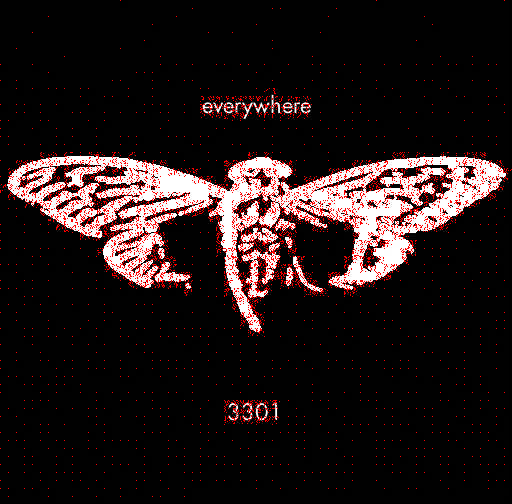
\includegraphics[scale=0.3]{agrippa_data_coefficients}
	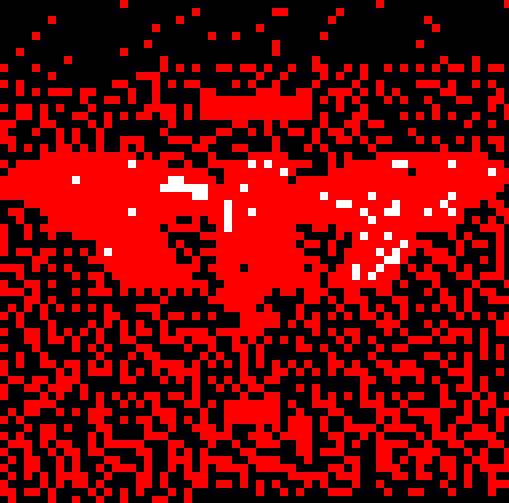
\includegraphics[scale=0.3]{agrippa_data_blocks}
	
	\caption{Agrippa variant}
\end{figure}

\begin{figure}[h]
	\centering
	
	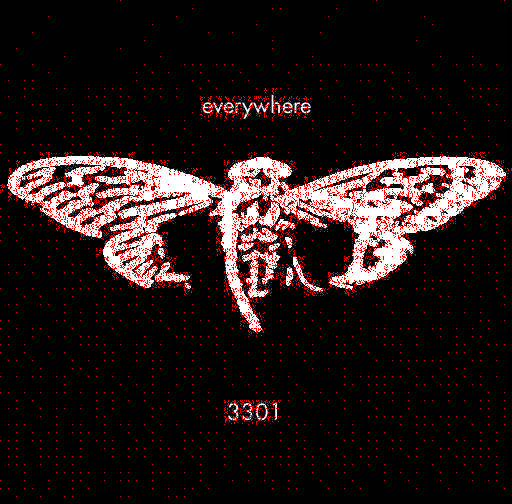
\includegraphics[scale=0.3]{brittanica_data_coefficients}
	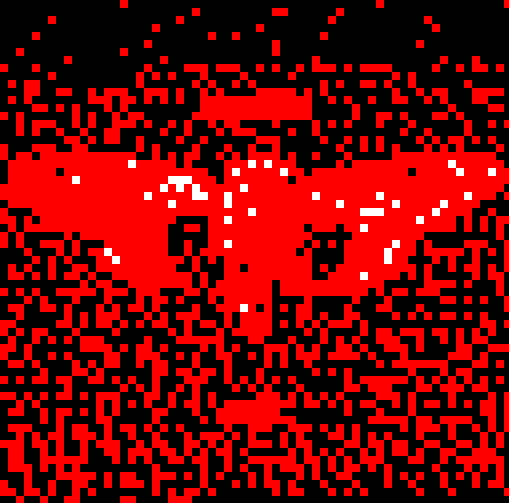
\includegraphics[scale=0.3]{brittanica_data_blocks}
	
	\caption{Brittanica variant}
\end{figure}
\FloatBarrier

Note that if a block is known to hold message data, it doesn't necessarely mean it will be modified (if the data it hold coincide with its data). \\

However, if a block is known to have been modified and isn't known to hold data bits, it means that one of its coefficient has been used either for statistical foiling purposes or to hide another message.

Assuming the original image prior to embedding had an entirely black background, we can infer that before the message was embedded, blocks of $8 \times 8$ black pixels were encoded as a constant color, with all other coefficients being otherwise zero.

In such a block, the single coefficient whose value isn't 0 or 1 is the coefficient of the constant term. Consequently, if such a block is used to embed a bit, the output block will simply be uniformly colored-block, with a slightly different color.

Based on the assumption mentioned above, we can detect blocks of blacks pixels that have been modified to embed bits. In both images, the color of unmodified black blocks is $\#010101$. The color of modified blocks is $\#000000$.

\begin{figure}[h]
	\centering
	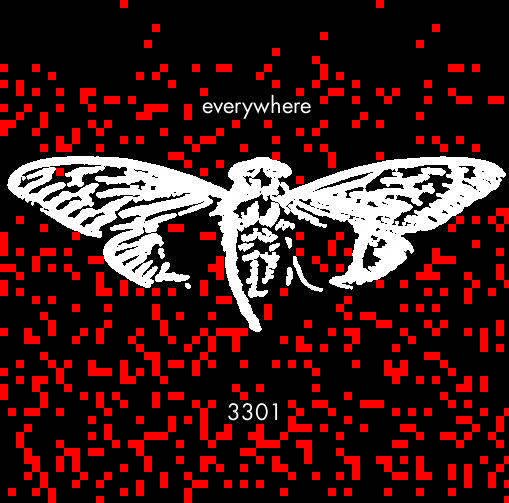
\includegraphics[scale=0.3]{agrippa_black_modifications_detected}
	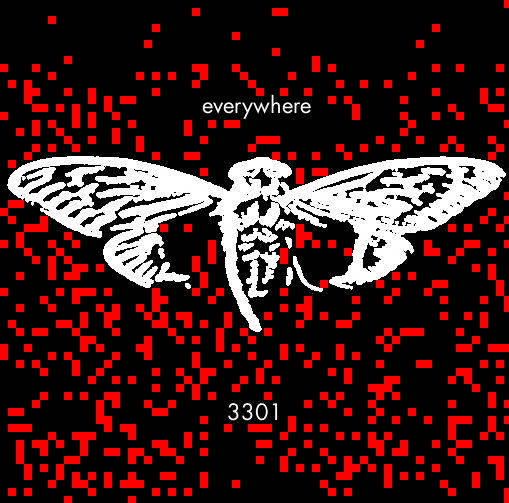
\includegraphics[scale=0.3]{brittanica_black_modifications_detected}
	
	\caption{Modified black blocks detected -- Left: Agrippa, Right: Brittanica}
\end{figure}

Interestingly, all but two block modifications observed can be explained by the data embedding pattern.

Many black blocks observed to have been modified cannot be explained simply by message embedding process alone. These two blocks are in the lower right corner in each image :

\begin{figure}[h]
	\centering
	
	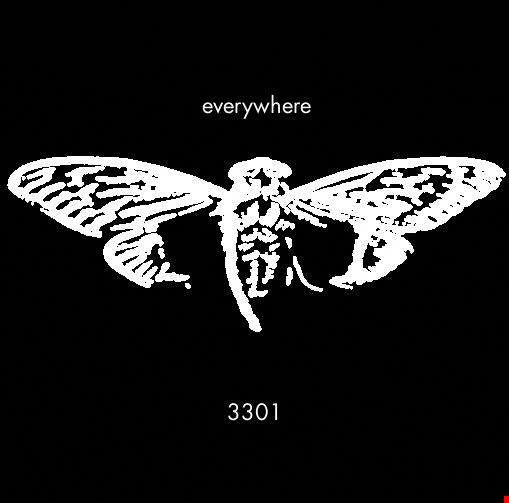
\includegraphics[scale=0.3]{agrippa_non_embedding_changes}
	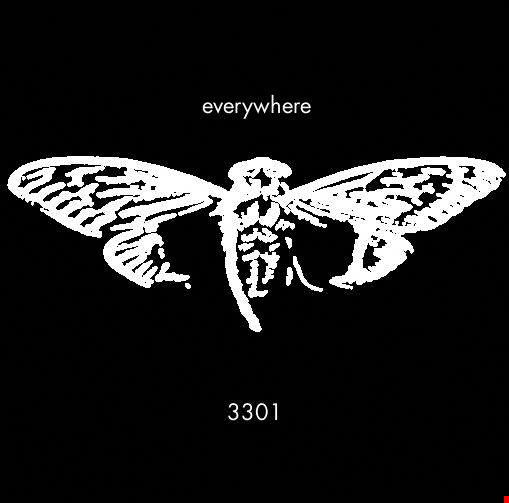
\includegraphics[scale=0.3]{brittanica_non_embedding_changes}
	
	\caption{Modifications observed unexplainable solely using the data bits embedding process -- Left: Agrippa variant, Right: Brittanica variant}
\end{figure}

This means that either a second data file is also embedded or that statistical foiling is enabled (or both).

\paragraph{Is a second message embedded ?}

If a second message is embedded in one of the two images, then all of its bits must have been stored in the LSB of DCT coefficients not used to store the first message. This second message will use at the very least -- in the case of a message of length zero -- 32 DCT coefficients to store its header.

Next up, we'll compute the probability for its header to have been hidden in such a way that it wouldn't be detectable by only looking at the modified $8 \times 8$ black pixels blocks. \\

Initialization of the RC4 stream used as part of the bit selection algorithm involves computing a MD5 digest of the user-supplied key. Consequently, it wouldn't be computationally feasible for 3301 to have bruteforced a key such that the second message would be hidden being undetectable by looking at the modified black blocks. This observation legitimates the computation of the above probability. \\

We'll make the hypothesis that RC4 streams are random. \\

Computing the exact probability is difficult, as there are about $32^{32}$ different ways the DCT coefficients can be chosen. For each choice of coefficients, we would need to count how many black blocks could be modified. Instead, we will compute an upper-bound by only looking at the first $20$ bits of the header data. \\

In both "everywhere" images, the first usable DCT coefficient which doesn't correspond to a black $8 \times 8$ pixel block is the 708th. 

The offset between two consecutive positions of the bitmap iterator is uniformly chosen in the range $\{ 1, \ldots, 32 \}$. The iterator starts on the offset uniformly chosen in $\{ 0, \ldots, 31\}$. The coefficient possible DCT coefficient to be used to embed the first 20 bits header bits is the $32\times20 = 640$th.

Thus, the first 20 header bits will always be embedded in DCT coefficients corresponding to black $8 \times 8$ pixel blocks. For these 20 header bits to have been embdedded in a undetectable way, the LSB stored in these coefficients shouldn't change the coefficient value. That is to say, the $16$ bits from the RC4 stream used to encode the header data have to equal to a specific sequence of $16$ bits. This event will occur with the probability : \[
	p = \left(\frac 1 2\right)^{20} \approx 9.53 \times 10^{-7}
\]

This probability is very low. The probability for the entire $32$ bit header is even lower. \\

Consequently, \textbf{it is very unlikely that a second message is embedded in any of the two "everywhere" images}.

\paragraph{Statistical foiling} If the assumptions made are correct, statistical foiling has to be enabled.

One might have expected more blacks blocks to be modified by statistical foiling. However, such a block would be modified only to correct the transformation of a coefficient with value $-128$ to the value $-127$, if, after embedding the message data, there are more coefficients with value $-128$ than with value $-127$ compared to the source image. Assuming the image had an entirely black background, there would have been substantially more coefficients equal to $-127$ than to $-128$.

Furthermore, the last DCT coefficient being changed in both images can be explained by the final pass of the statistical foiling algorithm. Once the image has finished embedding its data, a second pass is done to try to modify DCT coefficients that couldn't be foiled in the first phase. For each coefficient value, the search is started from the end of the DCT coefficient list, in reverse order. The first suitable coefficient is chosen. This could explain why, for both images, the last usable coefficient (corresponding to the lower-right black $8 \times 8$ pixel block) was modified.

Consequently, \textbf{its is likely that statistical foiling was enabled for both "everywhere" images}. \\

Based on these observations, the different command line options related to embedding a second file weren't used (\texttt{-E}, \texttt{-D}, \texttt{-K}, \texttt{-x}), and statistical foiling was enabled (as it is by default) : \texttt{-F-} wasn't used.

\subsection{Do the images come from the same source image?}

As the operation of flipping the LSB maps $0$ to $1$ and the other way around, the data embedding and statistical foiling step won't change the number of DCT coefficients available. Both images have $29615$ usable DCT coefficients. 

DCT coefficients can be thought of as being organised in $(x, y)$ pairs, where changing the LSB of $x$ gives $y$ and the other way around. Let $n_x$ and $n_y$ be the number of such coefficients in an image. Embedding a message using Outguess shouldn't change the value $n_x + n_y$. It can be observed that for each $8 \times 8$ blocks, this sum is the same for all such pairs for both images.

These observations were made using the \texttt{pairs\_histogram} tool. \textbf{These are indications that both images originate from the same source image}. \\

\subsection{Reconstructing one possible source image}

Due to the simplicity of the "everywhere" images, reconstructing a possible source image can be attempted. We'll assume the source images (before the JPEG compression and embedding introduced some artifacts) are composed of a completely black background, and that the Cicada 3301 logo was overexposed to the point that it would only be composed of white pixels. By carefully rotoscoping the logo, both elements can be recreated quite easily.

\begin{figure}[h]
	\centering
	
	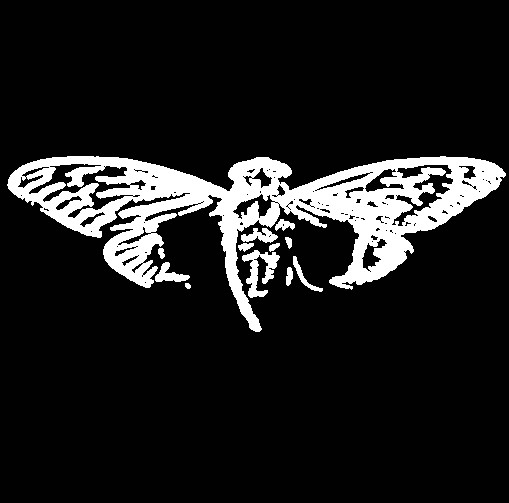
\includegraphics{partial_reconstruction}
	
	\caption{Partial image source reconstruction}
\end{figure}
\FloatBarrier

3301 could have used a JPEG or an PNM image as input for Outguess. As the JPEG format isn't lossless, the input file format matters for the recreation. \\

Our partial recreation lacks the two texts, which will severely modify the number of usable DCT coefficients. However, the JPEG compression algorithm works locally on $8 \times 8$ pixels blocks. We can thus just work on a part of the image assumed to have been perfectly recreated, such as the cicada. Note that have to make sure to stay aligned with the $8 \times 8$ grid.

\begin{figure}[h]
	\centering
	
	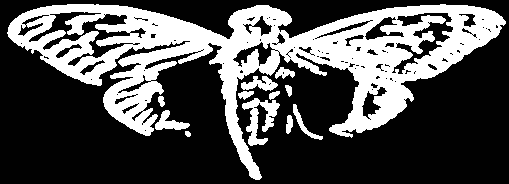
\includegraphics[scale=0.3]{partial_cicada_reconstruction}
	
	\caption{Subimage used for further analysis}
\end{figure}
\FloatBarrier

We'll use in parallel the corresponding subimages in the two "everywhere" variants.

To test whether 3301 used a PNM source image, we can run the JPEG compression algorithm with a quality of $75$ on the cicada recreation. If the resulting DCT coefficients different from what is observed in the "everwhere" images (ignoring the LSBs), it necessarily means that the source pixels aren't correct: because we assumed our recreation to be perfect, it means that JPEG was used instead of PNM which compressed the images.

This process has been automated by the tool \texttt{is\_pnm\_source}. \textbf{3301 probably didn't use a PNM source image.} \\

Consequently, 3301 must have used a JPEG source image. This lead us to make the hypothesis that the source pixels have been compressed twice: once when 3301 saved them as a JPEG image to use as an input to Outguess, a second time when Outguess recompressed it using a quality factor of $75$. The first quantization matrix used is unknown, we'll now attempt to determine it. \\

The default quantization algorithm implemented in the \texttt{libjpeg-6b} and consequently used by Outguess is:
\begin{minted}[fontsize=\footnotesize]{C}
short do_quantization(int unquantized_dct, int divisor) {
    int dct = unquantized_dct;

    if (dct < 0) {
        dct = -dct;

        dct += divisor >> 1;

        if (dct >= divisor)
            dct /= divisor;
        else
            dct = 0;

        dct = -dct;
    }
    else {
        dct += divisor >> 1;

        if (dct >= divisor)
            dct /= divisor;
        else
          dct = 0;
    }

    return dct;
}
\end{minted}

The quantization matrices used for the last compression (with a quality of $75$) are :
\begin{center}
	\[
		\begin{pmatrix}
			8 & 6 & 5 & 8 & 12 & 20 & 26 & 31 \\
			6 & 6 & 7 & 10 & 13 & 29 & 30 & 28 \\
			7 & 7 & 8 & 12 & 20 & 29 & 35 & 28 \\
			7 & 9 & 11 & 15 & 26 & 44 & 40 & 31 \\
			9 & 11 & 19 & 28 & 34 & 55 & 52 & 39 \\
			12 & 18 & 28 & 32 & 41 & 52 & 57 & 46 \\
			25 & 32 & 39 & 44 & 52 & 61 & 60 & 51 \\
			36 & 46 & 48 & 49 & 56 & 50 & 52 & 50 \\
		\end{pmatrix}
	\]
	Luminance quantization table \\
	\[
		\begin{pmatrix}
			9 & 9 & 12 & 24 & 50 & 50 & 50 & 50 \\
			9 & 11 & 13 & 33 & 50 & 50 & 50 & 50 \\
			12 & 13 & 28 & 50 & 50 & 50 & 50 & 50 \\
			24 & 33 & 50 & 50 & 50 & 50 & 50 & 50 \\
			50 & 50 & 50 & 50 & 50 & 50 & 50 & 50 \\
			50 & 50 & 50 & 50 & 50 & 50 & 50 & 50 \\
			50 & 50 & 50 & 50 & 50 & 50 & 50 & 50 \\
			50 & 50 & 50 & 50 & 50 & 50 & 50 & 50 \\
		\end{pmatrix}
	\]
	Chrominance quantization table
\end{center}

Using the algorithm and tables above, we can compute for each coefficient of the two "everywhere" variants  subimages all values it could have had before its quantization. Note that we have also to consider for each DCT coefficient a second version where the LSB is flipped -- as some coefficients where modified by the data embedding algorithm. \\

There are also 3 (unknown) quantization tables associated with the first quantization introduced by 3301 using a JPEG image as the input to Outguess. However, virtually all JPEG images use the same tables for both chrominance channels. Consequently, we're only looking for two matrices -- $(l_{i, j})_{1 \le i, j \le 8}$ and $(c_{i, j})_{1 \le i, j \le 8}$. \\

Assuming our recreation of the cicada to be correct, it can be used to add contraints of the coefficients of the two matrices. There constraints result in the following quantization tables:

\begin{table}
\end{table}

\bibliographystyle{plain}
\bibliography{bibliography}

\end{document}
